\documentclass{article}

\usepackage[utf8]{inputenc}
\usepackage{graphicx}
\usepackage{lipsum}

\makeatletter
    \setlength\@fptop{0\p@}
\makeatother


\begin{document}
\setcounter{secnumdepth}{0}
\section{Control dinámico}

Se realizó el control dinámico del robot utilizando Simscape. El modelo completo puede observarse en la Figura 1. Los bloques trayectorias definen los perfiles de posiciones que debe seguir cada pata del robot. Cada una de las elementos(muslo, pierna y cuerpo del robot) poseen una masa y momento de inercia deteminado por las dimensiones de la estructura y ubicaciones de las masas involucradas. Se utilizan lazos PID como método de control de posición que pueden ser facilmente observados en la Figura 2. 

\begin{figure}[!h]
  \centering
  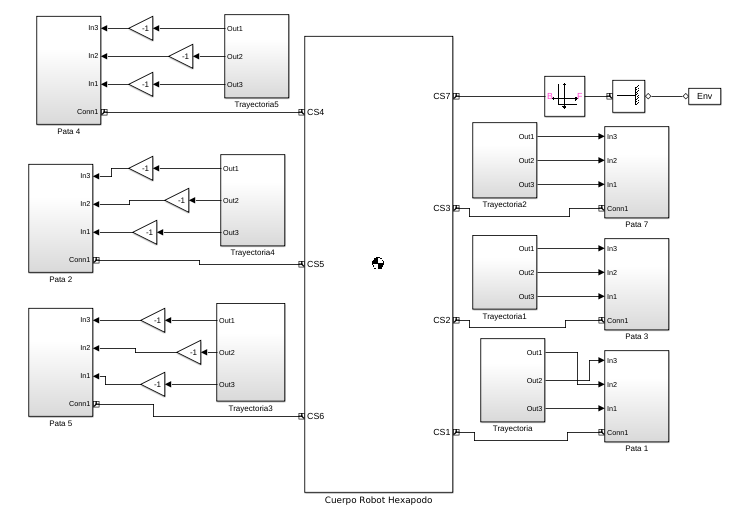
\includegraphics[width=1\linewidth]{hex.png}
  \caption{Modelo dinámico total}
\end{figure}

\begin{figure}[!h]
  \centering
  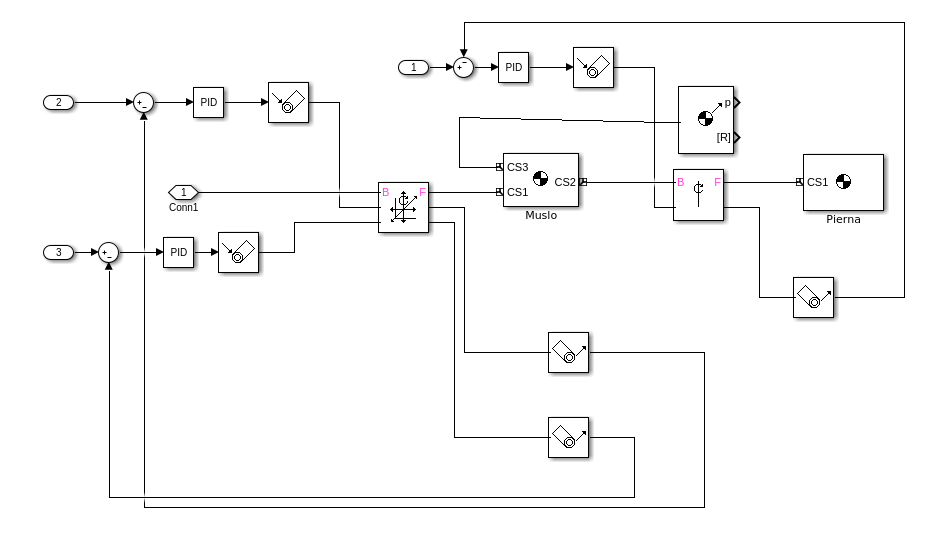
\includegraphics[width=1\linewidth]{leg.png}
  \caption{Modelo dinámico de una pierna}
\end{figure}



\end{document}